%version of 08-15-19

\chapter{$\oplus$ Wondrous Applications of Fibonacci Numbers}
\label{ch:FIBO-enrich}

\section{$\oplus$ Computing Products of Consecutive Fibonacci Numbers}
\label{sec:product-Fn-Fn+1}
\index{Fibonacci numbers!product of consecutive}

One feature of the Fibonacci numbers that has captivated an entire
community of mathematically oriented people is the plethora of simply
presented identities involving the numbers.\footnote{Indeed, an entire
  research journal, {\it The Fibonacci Quartlerly},\index{The
    Fibonacci Quartlerly} is dedicated to the mathematics of Fibonacci
  numbers and their kin, including the sharing of such identities.}
We now present a particularly beautiful identity.

\begin{prop} 
\label{thm:FiboSumConsecutive}
For all $n \geq 1$,
\begin{equation}
\label{eq:FiboSumConsecutive}
F(n) \cdot F(n-1) \ \ = \ \ \sum_{k=0}^{n-1} (F(k))^2.
\end{equation}
\end{prop}

\begin{proof}
One can observe identity (\ref{eq:FiboSumConsecutive}) ``in action''
in Fig.~\ref{fig:fibosquare}.  We augment this visual validation of
the identity with the following induction.

\medskip

\noindent {\it Base case.}
Instance $n=1$ of identity (\ref{eq:FiboSumConsecutive}) is valid
because
\[ F(0) \cdot F(1) \ = \ 1 \cdot 1 \ = \ 1^2 \ = \ (F(0))^2. \]

\medskip

\noindent {\it Inductive hypothesis.}
Assume that identity (\ref{eq:FiboSumConsecutive}) is valid for all $n
\leq m$.

\medskip

\noindent {\it Inductive extension.}  Let us focus on the product
$F(m+1) \cdot F(m)$.  Invoking the defining Fibonacci recurrence
(\ref{eq:Fibonacci-defn}) and the inductive hypothesis, we generate
the following chain of identities.
\begin{eqnarray*}
F(m+1) \cdot F(m)
 & = &
   (F(m) + F(m-1)) \cdot F(m) \\
 & = &
   (F(m))^2 + \big( F(m) \cdot F(m-1) \big) \\
 & = & 
   (F(m))^2 + \big( \sum_{k=0}^{m-1} (F(k))^2 \big) \\
 & = &
   \sum_{k=0}^{m} (F(k))^2.
\end{eqnarray*}
The induction is thus extended, which completes the proof.
\qed
\end{proof}


\section{$\oplus \oplus$ A Number System Based on the Fibonacci Sequence}
\label{sec:numerals-special-families}
\label{sec:Fibo-numbers}


\subsection{Preliminaries}
{\Denis write a short introduction here}

In a variety of application areas, the special properties of certain
families of numbers can be exploited if one uses the numbers in the
family to devise representations of all integers.  We illustrate this
fact while using the Fibonacci numbers---see
Section~\ref{sec:Fibonacci}---as our basis family.

We shall repeatedly find the following nonstandard notation useful:

For integers $m$ and $n$, we write $[m \gg n]$ to mean that $m \geq
n+2$.

\medskip


We will first prove the \textit{Zeckendorf's theorem} which informally states
that every positive integer $n$ has a unique representation of the
form:  **CITATION**

$n = F(k_1) + F(k_2) + ... + F(k_r)$ where $k_1 \gg k_2 \gg ... \gg k_r$ and $k_r \geq 2$.

Here, we assume that the Fibonacci sequence starts at index $1$ and not $0$,
moreover, the decompositions will never consider $F(1)$ (since $F(1)=F(2$)). 
For instance, the representation of $12345$ turns out to be:

$12345 = 10946 + 987 + 377 + 34 + 1 = F(21) + F(16) + F(14) + F(9) + F(2)$
\bigskip

Figure~\ref{zeckendorf} shows the decomposition of the first 26 integers written in this system. 
\begin{figure}[h]
\begin{center}
%\includegraphics[width=0.4\textwidth]{../FIGmaths/zeckendorf_representations.png}
        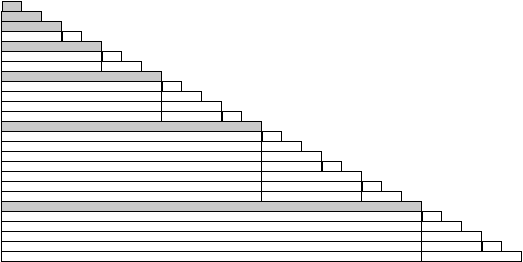
\includegraphics[scale=0.6]{FiguresArithmetic/Zeckendorf}
        \caption{The first integers (on the Y-axis) broken down into the Zeckendorf representation.
        The shaded rows corresponds to pure Fibonacci numbers.}
\label{zeckendorf}
\end{center}
\end{figure}

\subsection{Proof of Zeckendorf's Theorem}

The proof is done by induction on $n$ for proving simultaneously both construction and uniqueness.

\begin{itemize}
\item
The basis is true since the decomposition is obviously unique for $n=2$ (and also for $n=3$). 
Notice that for $n=4$, we have $4 = 3 + 1 = F(4) + F(2)$. 

\item
Assume for the induction step that any integer strictly lower than $F(k)$ can be decomposed uniquely as the sum of non-consecutive Fibonacci numbers.
We will prove as a consequence that an integer $n$ in the next interval between two consecutive Fibonacci numbers $F(k) \leq n < F(k+1)$ may be decomposed. 

If $n=F(k)$ is a Fibonacci number, the decomposition is reduced to $F(k)$.

Moreover, it is not difficult to check that it is unique.

%by using Property~\ref{prop:FiboSum}:
%$F(k) = 2+ \sum_{i=1}^{k-2} F(i)$ (the 2 comes from the shift of the starting element of the sequence...).

\medskip

If $n \neq F(k)$ write $n = F(k) + N$.

As $N$ is strictly lower than $F(k)$, we apply the recurrence hypothesis to decompose it into non-consecutive Fibonacci numbers:

$n = F(k) + F(k_1) + F(k_2) + \cdots + F(r)$ where $k_2 \gg ... \gg k_r \geq 2$. 

The last point to verify is that $F(k)$ and $F(k_1)$ are not consecutive ($F(k) \gg F(k_1)$), which is done by contradiction:

Assuming $k$ and $k_1$ are consecutive ($k_1=k-1$) leads to $n = F(k+1) + F(k_2) + \cdots + F(r)$
which contradicts $n < F(k+1)$.
\end{itemize}


\subsection{Applications of the FIBO number system}

Any unique system of representation is a numbering system.

The previous theorem ensures that any non-negative integer can be written
as a sequence of bits $b_i$, in other words,

$n = (b_mb_{m-1}...b_2)_F$ iff $n = \Sigma_{k=2}^m b_k F(k)$.

Note: we wrote here the representation of $n$ in the Fibonacci numbering system using parenthesis in order to avoid confusions 
on the indices.

Let us compare this system to the binary representation.
For instance, the Fibonacci representation of $12345$ is $100001010000100000010_F$
while  $12345 = 2^{13} + 2^{12} + 2^{5} + 2^{4} + 2^{3} + 2^{0} = 1100000111001_2$.
The binary representation is more compact. 
\bigskip

The decomposition in the Fibonacci basis of the first integers (starting from $1 = 00001_F$) is as follows:

 $2 = 0010_2 = F(3) = 00010_F$
 
 $3 = 0011_2 = F(4) = 00100_F$
  
 $4 = 100_2 = 3+1 = 00101_F$
 
 $5 = 101_2 = F(5) = 01000_F$
 
 $6 = 110_2 = 5+1 = 01001_F$
 
 $7 = 111_2 = 5+2 = 01010_F$
 
 $8 = 1000_2 = F(6) = 10000_F$
 
 $9 = 1001_2 = 10001_F$
 
 $10 = 1010_2 = 10010_F$
 
 $11 = 1011_2 = 10100_F$
 
 $12 = 1100_2 = 10101_F$
 
 $13 = 1101_2 = F(7) = 100000_F$
 
 ...
 
There is no consecutive digits equal to $1$ in such representations.
\medskip

{\Denis I can write briefly how to perform an addition within this system, what do you think?}
{\Arny Definitely yes}



\section{$\oplus \oplus$ Greatest Common Divisors of Fibonacci Numbers}
\label{Appendix:FiboGCD}

This is a draft, in particular, the notation should be put in coherency with the other chapters
($F(n)$ instead of $F_n$)
\bigskip

Let $F_1=F_2=1$ and $F_{n+1}=F_n+F_{n-1}$.
\medskip

\noindent We want to prove that $GCD(F_n,F_m) = F_{GCD(n,m)}$.
{\Denis put it like a proposition?}

Without loss of generality, consider that $n \geq m$.

Check the property on particular cases (gain intuition)...

Let us denote $g=GCD(n,m)$ and $G=GCD(F_n,F_m)$.

As an example, let us check 

$GCD(F_{12},F_{18}) = GCD(144,2584) = 8 = F_6$ (where $6=GCD(12,18)$).
\medskip

This result is obtained by showing first that $F_g$ divides $G$ and then, $G$ divides $F_g$.

Let us first prove three technical lemmas.
\\

\noindent {\bf Lemma 1.}
The following relation holds for any integers $n$ and $k$:

$F_{n+k} = F_k.F_{n+1} + F_{k-1}.F_n$ \footnote{this relation assumes that we are able to define negative Fibonacci numbers. 
Well, there is a "natural" way of extending
the definition to negative numbers...}

The proof is straightforward  by induction on $k$ assuming that $n$ is fixed.
\\

\noindent {\bf Lemma 2.}
For any integer $k$ $F_{k.n}$ is a multiple of $F_n$.

The proof can be obtained as a consequence of the previous lemma.
\\

\noindent {\bf Lemma 3.}
If $a$ divides $b$ then $F_a$ divides $F_b$.
\\

We are able now to prove the final result:
\begin{enumerate}
\item $F_g$ divides $G$.

By definition of the GCD, $g$ divides $n$ and $m$. 
Using Lemma 3, that means that $F_g$ divides both $F_n$ and $F_m$.
thus, it divides their GCD.
\item $G$ divides $F_g$.

As $g$ is the GCD of $n$ and $m$, it can be written as a linear combination of them (in fact it is the smallest one):
$g = a.n + b.m$.

$F_g = F_{a.n + b.m}$ for some integers $a$ and $b$,
thus, according to lemma 1, it is a multiple of $n$ (and symmetrically of $m$).
Thus, it is a multiple of their GCD. 
\end{enumerate}






